%xelatex
\documentclass[14pt,]{extreport}

\usepackage[T2A]{fontenc}
\usepackage[utf8]{inputenc}
\usepackage[english,ukrainian]{babel}
%\usepackage{fontspec}
\usepackage{amsmath}
\usepackage{mathtools}
\usepackage{caption}
\usepackage{diagbox}
\usepackage{tikz}
\usetikzlibrary{tikzmark}
\usepackage{mathspec}
\setallmainfonts{Nimbus Roman}
\usepackage{graphicx}
\usepackage[a4paper,margin=0.5in]{geometry}
\usepackage{pgfplots}
\pgfplotsset{width=10cm,compat=1.8}
\usepackage{indentfirst}
\usepackage{boxedminipage}
\usepackage{wrapfig}
\usepackage{subfiles}

\begin{document}
\pagestyle{empty}

\subfile{title}

\subsubsection*{Мета роботи}

Мета роботи – ознайомитись на практиці із застосуванням логіки
висловлювань у програмній інженерії, навчитись будувати досконалі кон’юктивну
та диз’юктивну форми, мінімізувати їх за допомогою карт Карно.

\begin{center}\bf Варіант 12\end{center}

\subsubsection*{1. Записати досконалу диз’юнктивну нормальну
форму та досконалу кон’юнктивну нормальну форму формул
$f_1(x_1,x_2,x_3), f_2(x_1,x_2,x_3),\\ f_3(x_1,x_2,x_3)$ та $f_4(x_1,x_2,x_3),$
які задані таблицею істинності:}

\begin{center}
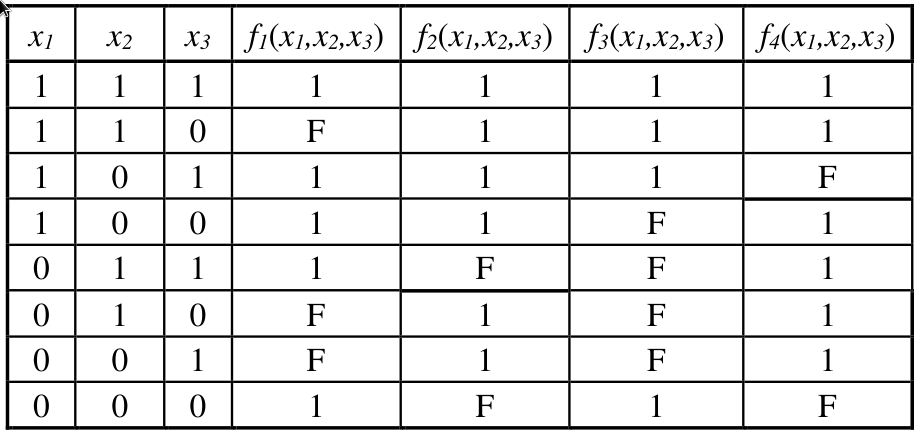
\includegraphics[width=.7\textwidth]{table.png}
\end{center}


\subsubsection*{ДДНФ:}
\subsubsection{$f_1(x_1,x_2,x_3)$}


$
(	x_1\land x_2\land x_3)\lor
(	x_1\land \bar x_2\land x_3)\lor
(	x_1\land \bar x_2\land \bar x_3)\lor
(	\bar x_1\land x_2\land x_3)\lor
(	\bar x_1\land \bar x_2\land \bar x_3)
$

\subsubsection{$f_2(x_1,x_2,x_3)$}

$
(	x_1\land x_2\land x_3)\lor
(	x_1\land x_2\land \bar x_3)\lor
(	x_1\land \bar x_2\land x_3)\lor
(	x_1\land \bar x_2\land \bar x_3)\lor
(	\bar x_1\land x_2\land \bar x_3)\lor
(	\bar x_1\land \bar x_2\land x_3)
$

\subsubsection{$f_3(x_1,x_2,x_3)$}
$
(	x_1\land x_2\land x_3)\lor
(	x_1\land x_2\land \bar x_3)\lor
(	x_1\land \bar x_2\land x_3)\lor
(	\bar x_1\land \bar x_2\land \bar x_3)
$

\subsubsection{$f_4(x_1,x_2,x_3)$}
$
(	x_1\land x_2\land x_3)\lor
(	x_1\land x_2\land \bar x_3)\lor
(	x_1\land \bar x_2\land \bar x_3)\lor
(	\bar x_1\land x_2\land x_3)\lor
(	\bar x_1\land x_2\land \bar x_3)\lor
(	\bar x_1\land \bar x_2\land x_3)
$

\begin{center}
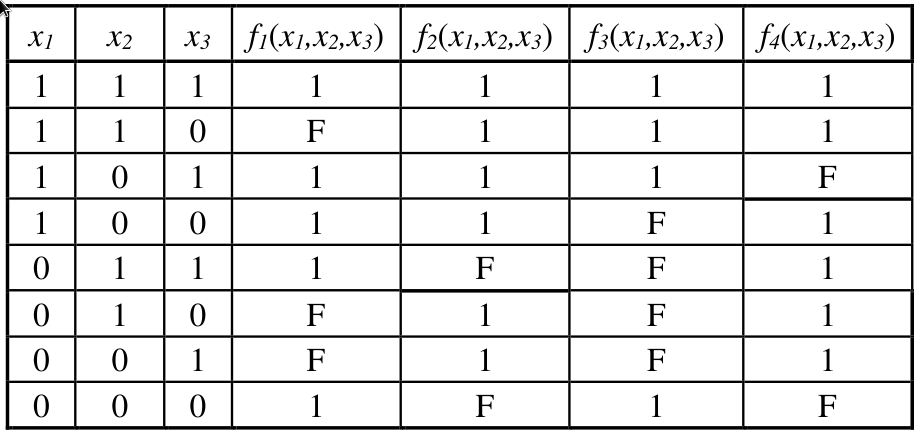
\includegraphics[width=.7\textwidth]{table.png}
\end{center}

\subsubsection*{ДКНФ:}

\subsubsection{$f_1(x_1,x_2,x_3)$}
$
(\bar x_1\lor \bar x_2 \lor x_3)\land
(x_1\lor \bar x_2\lor x_3)\land
(x_1\lor x_2\lor \bar x_3)
$
\subsubsection{$f_2(x_1,x_2,x_3)$}
$
(x_1\lor \bar x_2\lor \bar x_3)\land
(x_1\lor x_2\lor x_3)
$
\subsubsection{$f_3(x_1,x_2,x_3)$}
$
(\bar x_1\lor x_2\lor x_3)\land
(x_1\lor \bar x_2\lor \bar x_3)\land
(x_1\lor \bar x_2\lor x_3)\land
(x_1\lor x_2\lor \bar x_3)
$
\subsubsection{$f_4(x_1,x_2,x_3)$}
$
(\bar x_1\lor x_2\lor\bar x_3)\land
(x_1\lor x_2\lor x_3)
$
\medskip

\subsubsection*{2. За допомогою карт Карно мінімізувати функцію $\overline{pq}r\lor\overline{pqr}\lor\bar p \bar q r
\lor \bar p q \bar r \lor p\bar q\bar r$}

%\begin{tabular}{|c|c|c|c|c|c|}
%	\hline
%	\diagbox{r}{pq} & 00 & 01 & 11 & 10 \\
%	\hline
%	0 & $\overline{pqr}$
%	& $\bar p q \bar r$
%	& & $p \bar q \bar r$\\
%	\hline
%	1
%	& $\bar p \bar q r$ & & &\\
%	\hline
%\end{tabular}

\bigskip
\begin{tabular}{|c|c|c|c|c|c|}
	\hline
	& $qr$ & $q\bar r$ & $\bar q\bar r$ & $\bar q r$\\
	\hline
	$p$ & & & \tikzmark{startup} x &\\
	\hline
	$\bar p$ & &\tikzmark{startdown} x &\tikzmark{start3}
	 x \tikzmark{endup}
	\tikzmark{enddown} & x\tikzmark{end3}\\
	\hline
\end{tabular}

\begin{tikzpicture}[remember picture,overlay]
\foreach \Val in {down,3}
{
\draw[rounded corners,red,thick]
  ([shift={(-0.5\tabcolsep,-0.5ex)}]pic cs:start\Val)
    rectangle
  ([shift={(0.5\tabcolsep,2ex)}]pic cs:end\Val);
}

\foreach \Val in {up}
{
\draw[rounded corners,red,thick]
  ([shift={(-0.5\tabcolsep,2.2ex)}]pic cs:start\Val)
    rectangle
  ([shift={(0.5\tabcolsep,-1.3ex)}]pic cs:end\Val);
}
\end{tikzpicture}

\bigskip
$\bar q \bar r \lor \bar p \bar r \lor \bar p \bar q$

\subsubsection*{Висновок}

Виконавши цю практичну роботу, я закріпив свої знання про
побудову ДДНФ та ДКНФ булевих функцій та застосування
методу карт Карно для їх мінімізації.

\end{document}
